\chapter{Results and Discussion}
\begin{tcolorbox}[title=Group Members]
    \begin{enumerate}
        \itemsep0em
        \item Nashwan Hafid Andayuri, 25/554944/PA/23251
        \item Mhs 2, NIM: 
        \item Mhs 3, NIM:
    \end{enumerate}
\end{tcolorbox}
\section{Entity Relationship Diagram}
From the analysis of the business processes and the given constraints, this section can explain several things, including: \textit{cardinality mapping}, relevant attributes and keys, etc.

The ER diagram for the Academic Database is shown in Figure \ref{gb:1}
\begin{figure}[!h]
    \centering
    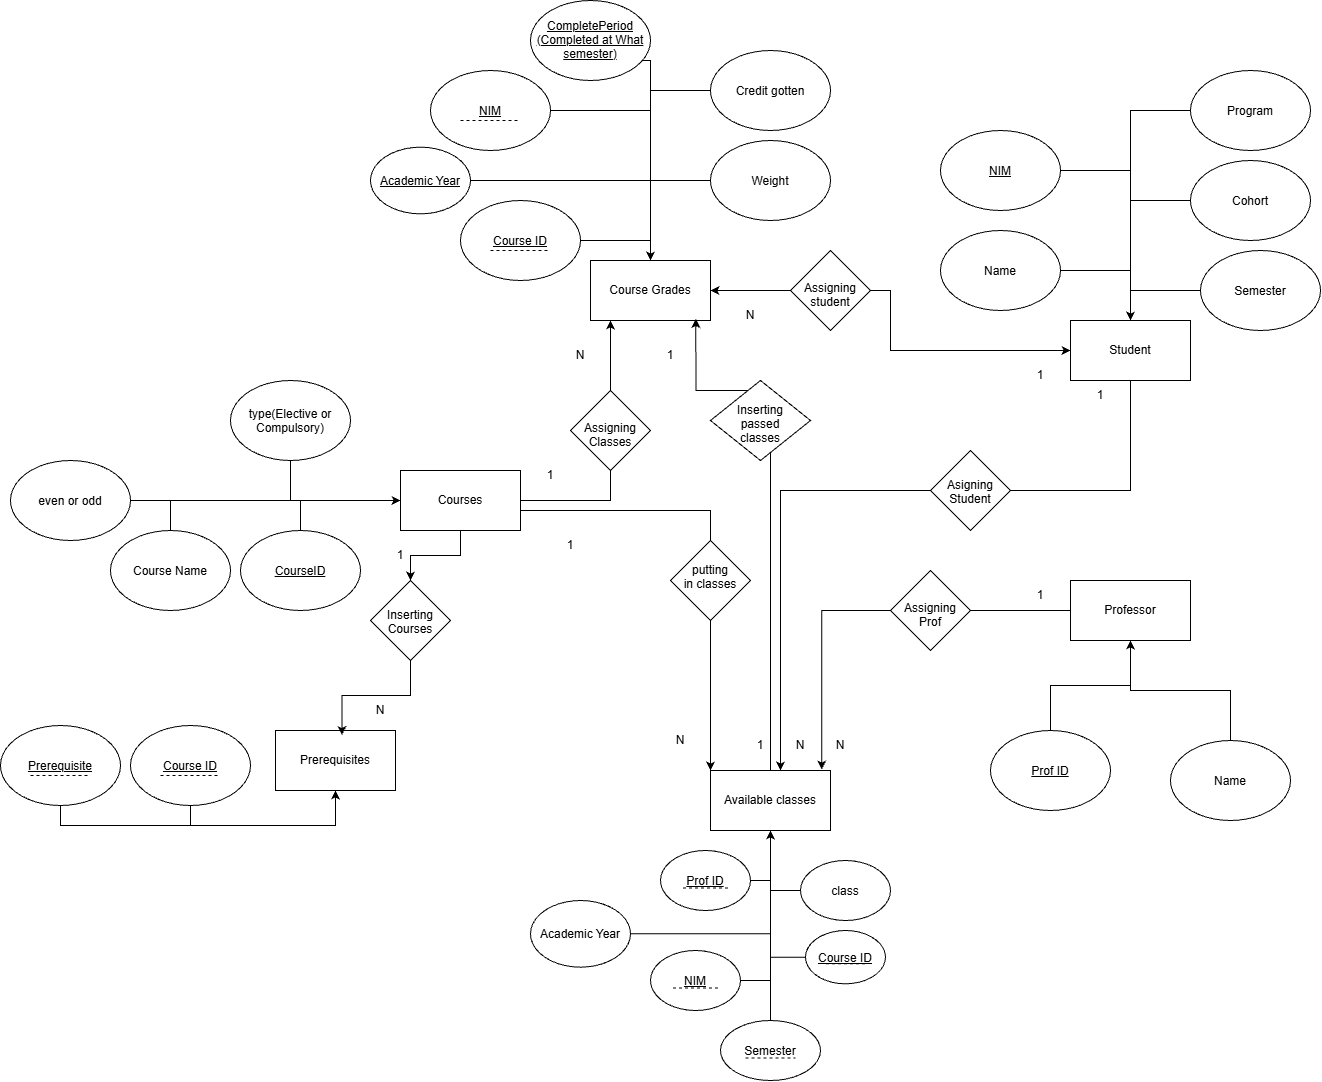
\includegraphics[width=.85\linewidth]{ERD.png}
    \caption{ER Diagram of the Academic Database}
    \label{gb:1}
\end{figure}
\section{Schema of Tables in the Database}
\begin{tcolorbox}[title=Table Schema in the Academic Database]
\begin{itemize}
    \itemsep0em
     \item \texttt{students(nim, name, semester, cohort, program)}
     \item \texttt{professors(prof id, name)}
      \item \texttt{courses(course name, course id, period, type, academic year)}
      \item \texttt{prerequisites(prerequisite, course id)}
      \item \texttt{AvailableClasses(prof id, nim, class, course id, semester, academic year)}
      \item \texttt{CourseGrades(course id, nim, academic year,completed period, credits, weight)}
      \item \texttt{CREATE TABLE students (
      	nim VARCHAR(20) PRIMARY KEY,
      	name VARCHAR(100) NOT NULL,
      	semester INT,
      	cohort VARCHAR(20),
      	program VARCHAR(100)
      	);
      	
      	CREATE TABLE professors (
      	prof_id VARCHAR(20) PRIMARY KEY,
      	name VARCHAR(100) NOT NULL
      	);
      	
      	CREATE TABLE courses (
      	course_id VARCHAR(20) PRIMARY KEY,
      	course_name VARCHAR(100) NOT NULL,
      	period VARCHAR(20),
      	type VARCHAR(50),
      	academic_year VARCHAR(20)
      	);
      	
      	CREATE TABLE prerequisites (
      	prerequisite VARCHAR(20),
      	course_id VARCHAR(20),
      	PRIMARY KEY (prerequisite, course_id),
      	FOREIGN KEY (prerequisite) REFERENCES courses(course_id),
      	FOREIGN KEY (course_id) REFERENCES courses(course_id)
      	);
      	
      	CREATE TABLE AvailableClasses (
      	prof_id VARCHAR(20),
      	nim VARCHAR(20),
      	class VARCHAR(20),
      	course_id VARCHAR(20),
      	semester INT,
      	academic_year VARCHAR(20),
      	PRIMARY KEY (prof_id, class, course_id, semester, academic_year),
      	FOREIGN KEY (prof_id) REFERENCES professors(prof_id),
      	FOREIGN KEY (nim) REFERENCES students(nim),
      	FOREIGN KEY (course_id) REFERENCES courses(course_id)
      	);
      	
      	CREATE TABLE CourseGrades (
      	course_id VARCHAR(20),
      	nim VARCHAR(20),
      	academic_year VARCHAR(20),
      	completed_period VARCHAR(20),
      	credits INT,
      	weight DECIMAL(3, 2),
      	PRIMARY KEY (course_id, nim, academic_year),
      	FOREIGN KEY (course_id) REFERENCES courses(course_id),
      	FOREIGN KEY (nim) REFERENCES students(nim)
      	);}
     
\end{itemize}  
\end{tcolorbox}
\section{Business Questions and Solutions Using SQL}
\subsection{Question number 1}
\begin{tcolorbox}
  \textit{List of elective course names and the courses that are their prerequisites (only name and course code information is sufficient). Courses that do not have prerequisites should still be displayed!}  
\end{tcolorbox}
\begin{enumerate}
    \itemsep0em
    \item Tables needed to answer the query:
    \item Join criteria (if any)
    \item SQL command according to the question
    \begin{lstlisting}
SELECT * FROM course where type='E'
    \end{lstlisting}
    \item Alternative SQL commands (if any) with adequate explanation
\end{enumerate}

\subsection{Question number 2}
\begin{tcolorbox}   
List of elective courses taken by Computer Science students of the '2024' cohort in the odd semester of academic year 2026/2027!
\end{tcolorbox}
\begin{enumerate}
    \itemsep0em
    \item Tables needed to answer the query:
    \item Join criteria (if any)
    \item SQL command according to the question
    \begin{lstlisting}
SELECT 
    FROM
    \end{lstlisting}
    \item Alternative SQL commands (if any) with adequate explanation
\end{enumerate}

\subsection{Question number 3}
\begin{tcolorbox}
    List of favorite elective courses for Computer Science students, namely the three courses with the most enrollees in the last three years!
\end{tcolorbox}
\begin{enumerate}
    \itemsep0em
    \item Tables needed to answer the query:
    \item Join criteria (if any)
    \item SQL command according to the question
    \begin{lstlisting}
SELECT 
    FROM
    \end{lstlisting}
    \item Alternative SQL commands (if any) with adequate explanation
\end{enumerate}

\subsection{Question number 4}
\begin{tcolorbox}
List of students who have a Semester Grade Point Average for the odd semester of 2025/2026 of no less than 3.25! (understand the difference between Semester GPA and Cumulative GPA)
\end{tcolorbox}
\begin{enumerate}
    \itemsep0em
    \item Tables needed to answer the query:
    \item Join criteria (if any)
    \item SQL command according to the question
    \begin{lstlisting}
SELECT 
    FROM
    \end{lstlisting}
    \item Alternative SQL commands (if any) with adequate explanation
\end{enumerate}

\subsection{Question number 5}
\begin{tcolorbox}
    List of students and the Cumulative GPA they have obtained to date! (courses that have been retaken only need to be counted once) 
\end{tcolorbox}
\begin{enumerate}
    \itemsep0em
    \item Tables needed to answer the query:
    \item Join criteria (if any)
    \item SQL command according to the question
    \begin{lstlisting}
SELECT 
    FROM
    \end{lstlisting}
    \item Alternative SQL commands (if any) with adequate explanation
\end{enumerate}